\documentclass[11pt]{article} % Font size (can be 10pt, 11pt or 12pt) and paper size (remove a4paper for US letter paper)

\usepackage{amsmath,amssymb,amsthm,gensymb}

\usepackage{geometry}
\usepackage{wrapfig}
\usepackage{hyperref}
\usepackage{makecell}

\hypersetup{
    colorlinks=true,
    linkcolor=black,
    filecolor=magenta,      
    urlcolor=blue,
}
\usepackage[protrusion=true,expansion=true]{microtype} % Better typography
\usepackage{hyperref}
\usepackage{graphicx} % Required for including pictures
\usepackage{wrapfig} % Allows in-line images
\linespread{1.12}
\usepackage{mathtools}
\usepackage[font=footnotesize,labelfont=bf]{caption}
\usepackage[T1]{fontenc} % Required for accented characters

\makeatletter

\newcommand{\bra}[1]{\left\langle #1 \right|}
\newcommand{\ket}[1]{\left|#1\right\rangle}
\newcommand{\braket}[2]{\left\langle#1 |  #2\right\rangle}
\makeatother



%\addbibresource{bibliography.bib}


\author{Francisca Vasconcelos\\\href{mailto:francisc@mit.edu} {francisc@mit.edu}}
\title{Introduction to Quantum Computing\\Lecture 6: Shor's and Grover's Algorithms}
\date{Massachusetts Institute of Technology\\6.s089 IAP 2020}

\begin{document}
\maketitle
\newpage
\tableofcontents
\newpage

\section{Shor's Algorithm}
Shor's algorithm, developed by now MIT Professor of Mathematics Peter Shor in 1994, is a polynomial-time quantum algorithm for integer factorization. This algorithm was of major significance for the field of quantum computation because it provided an exponential speedup for a very important problem. As it turns out integer factorization -- or moreso our inability to factor very large integers -- is the basis of RSA cryptography (an asymmetric cryptographic algorithm). Thus, Shor's algorithm gave an important motivation for the development of large-scale quantum computers.
\subsection{FT/QFT Review}
Last lecture, we discussed the Fourier Transform (FT) and its quantum counterpart, known as the Quantum Fourier Transform (QFT). As the FT maps signals in the time domain to the frequency domain, the QFT maps a quantum state to a superposition of states with frequency encoded in the state phases. 
\begin{equation*}
    U_{QFT}|j\rangle=\frac{1}{\sqrt{N}}\sum_{k=0}^{N-1}e^{2\pi ijk/N}|k\rangle
\end{equation*}
\begin{equation*}
    U_{QFT}=\frac{1}{\sqrt{N}}\sum_{j,k=0}^{N-1}e^{2\pi ijk/N}|k\rangle\langle j|
\end{equation*}
\newline
\newline
Another concept we need to review (or introduce depending on your signal processing background), is the FT of a delta train. We can define a delta train in the interval $\{0,M\}$ as follows,
\begin{equation*}
    f(x)=
    \begin{cases}
        \sqrt{\frac{r}{M}} \qquad \text{if } \quad x\equiv0 \pmod r \\
        \quad 2 \qquad\quad \text{otherwise}
    \end{cases}.
\end{equation*}
Its FT is thus defined as,
\begin{equation*}
    \hat{f}(x)=
    \begin{cases}
        \frac{1}{\sqrt{r}} \qquad \text{if } \quad x\equiv0 \pmod{\frac{M}{r}} \\
        \quad 0 \qquad\quad \text{otherwise}
    \end{cases}.
\end{equation*}
Thus, the FT of a delta train is simply another delta train (with potentially different spacings and amplitudes). This is important for our discussion of periodic functions, which can be generated from a convolution of a delta train with the period form of interest.

\subsection{Period Finding Algorithm}
We now discuss the period finding algorithm, which is a generalization of Simon's algorithm (1994). As it turns out, Shor's algorithm is simply a clever application of this algorithm to the problem of integer factorization, which turns out to be periodic in the domain of modular arithmetic. To begin, we will define the problem statement.
\newline\newline
\underline{Given}: black-box for computing a periodic function
\begin{equation*}
    f(x)=f(y) \text{ iff } x\equivy \pmod r
\end{equation*}
\underline{Goal}: find $r$
\newline\newline 
Classically, this would require querying the function with inputs until it repeats, giving an $O(r)=O(2^n)$ runtime (which has been proven to be exponential). In the quantum domain, however, we can access the function in a \textit{superposition} to query with $N=2^n$ inputs for each $n$ qubits at the same time (the key is the periodic and linear nature of the FT).
\newline\newline
Let's now work through the procedure of the period finding algorithm.
\newline\newline
\underline{Step 1: Prepare Periodic Superposition}
\newline\newline
We are going to start off our algorithm in the $\ket{0}\ket{0}$ state. Assume we are working with $N$ total qubits. The first step is to take the QFT of our first register,
\begin{equation*}
    \ket{0}\ket{0} \quad \overset{QFT_N}{\longrightarrow} \quad \frac{1}{\sqrt{N}}\sum_{x=0}^{N-1}\ket{x}\ket{0}
\end{equation*}
Note that this simply puts our first register into a uniform superposition over all $N$ quantum states. Given our $\ket{0}\ket{0}$ initialization, this could have also been achieved simply using Hadamards, $H^{\otimes n}$, instead of the QFT. 
\newline\newline
Let $U_f$ be a unitary encoding of our given black-box function $f$. For more information on how to create such a unitary, look into Simon's algorithm. We apply $U_f$ to our previously created state such that,
\begin{equation*}
    \frac{1}{\sqrt{N}}\sum_{x=0}^{N-1}\ket{x}\ket{0} \quad \overset{U_f}{\longrightarrow} \quad \frac{1}{\sqrt{N}}\sum_{x=0}^{N-1}\ket{x}\ket{f(x)} .
\end{equation*}
\newline\newline
In order to generate our desired periodic superposition state, we can simply measure the second register. This will cause $\ket{f(x)}$ to collapse to some $\ket{f(x_0)}$. Furthermore, measuring $\ket{f(x)}$ reveals information about $\ket{x}$, since $\ket{x}$ will be constrained to the pre-image of $\ket{f(x_0)}$. Because $f$ is periodic, the pre-image of $f(x_0)$ is $\{x_0, x_0+r, x_0+2r, ..., x_0+(\frac{N}{r}-1)r \}$. 
\begin{equation*}
    \frac{1}{\sqrt{N}}\sum_{x=0}^{N-1}\ket{x}\ket{f(x)} \quad \overset{\text{measure }f}{\longrightarrow} \quad  
    \sqrt{\frac{r}{N}}\sum_{i=0}^{N/r-1}\ket{ir+x_0}\ket{f(x_0)}.
\end{equation*}
Thus, our first register is in a periodic superposition with period of function $f$. Note, however, that we cannot simply measure the state of the first register. If we were to re-run the algorithm, we might measure a different value of $\ket{f(x)}$ and obtain a periodic superposition that is linearly shifted (i.e. different value of $x_0$). This means that we must find a way to eliminate the effect of the linear shift and generate a state which is solely dependent on the value of $r$.
\newline\newline
\underline{Step 2: Fourier Sample}
\newline\newline
Remember, if $f$ is periodic with period $r$ such that $\frac{N}{r}=k$, then $\hat{f}$ is periodic with period $k$. Furthermore, if $f$ has a linear shift of $x_0$, this is only visible in the phase of $\hat{f}$. Thus, if we take the FT of our first register, we will only be left with states that are multiples of $\frac{N}{r}$,
\begin{equation*}
    \sqrt{\frac{r}{N}}\sum_{i=0}^{N/r-1}\ket{ir+x_0}\ket{f(x_0)} 
    \quad \overset{QFT_N}{\longrightarrow} \quad 
    \frac{1}{\sqrt{r}}\sum_{i=0}^{r-1}\phi_i\ket{i\frac{N}{r}}\ket{f(x_0)}. 
\end{equation*}
Note that the linear shift is encoded in the phase $\phi_i$. If we measure the first register, we will retrieve $k\frac{N}{r}$ for some integer $k$. This means that in the case of repeated measurement, our outcome will not be altered dependent on the state $\ket{f(x)}$ collapses to.
\newline\newline
\underline{Step 3: Repeat \& GCD}
\newline\newline
In order to determine $r$, we must repeat steps 1 and 2 several times in order to retrieve distinct multiples of $\frac{N}{r}$. With enough values, we can compute their Greatest Common Divisor (GCD) using Euclid's algorithm, so as to retrieve $\frac{N}{r}$ itself. Since $N$ is given, once we have $\frac{N}{r}$, we can solve for $r$! 
\newline\newline
The overall algorithm runtime is $O(\log N)$ and the circuit goes as follows,
\begin{figure}
    \centering
    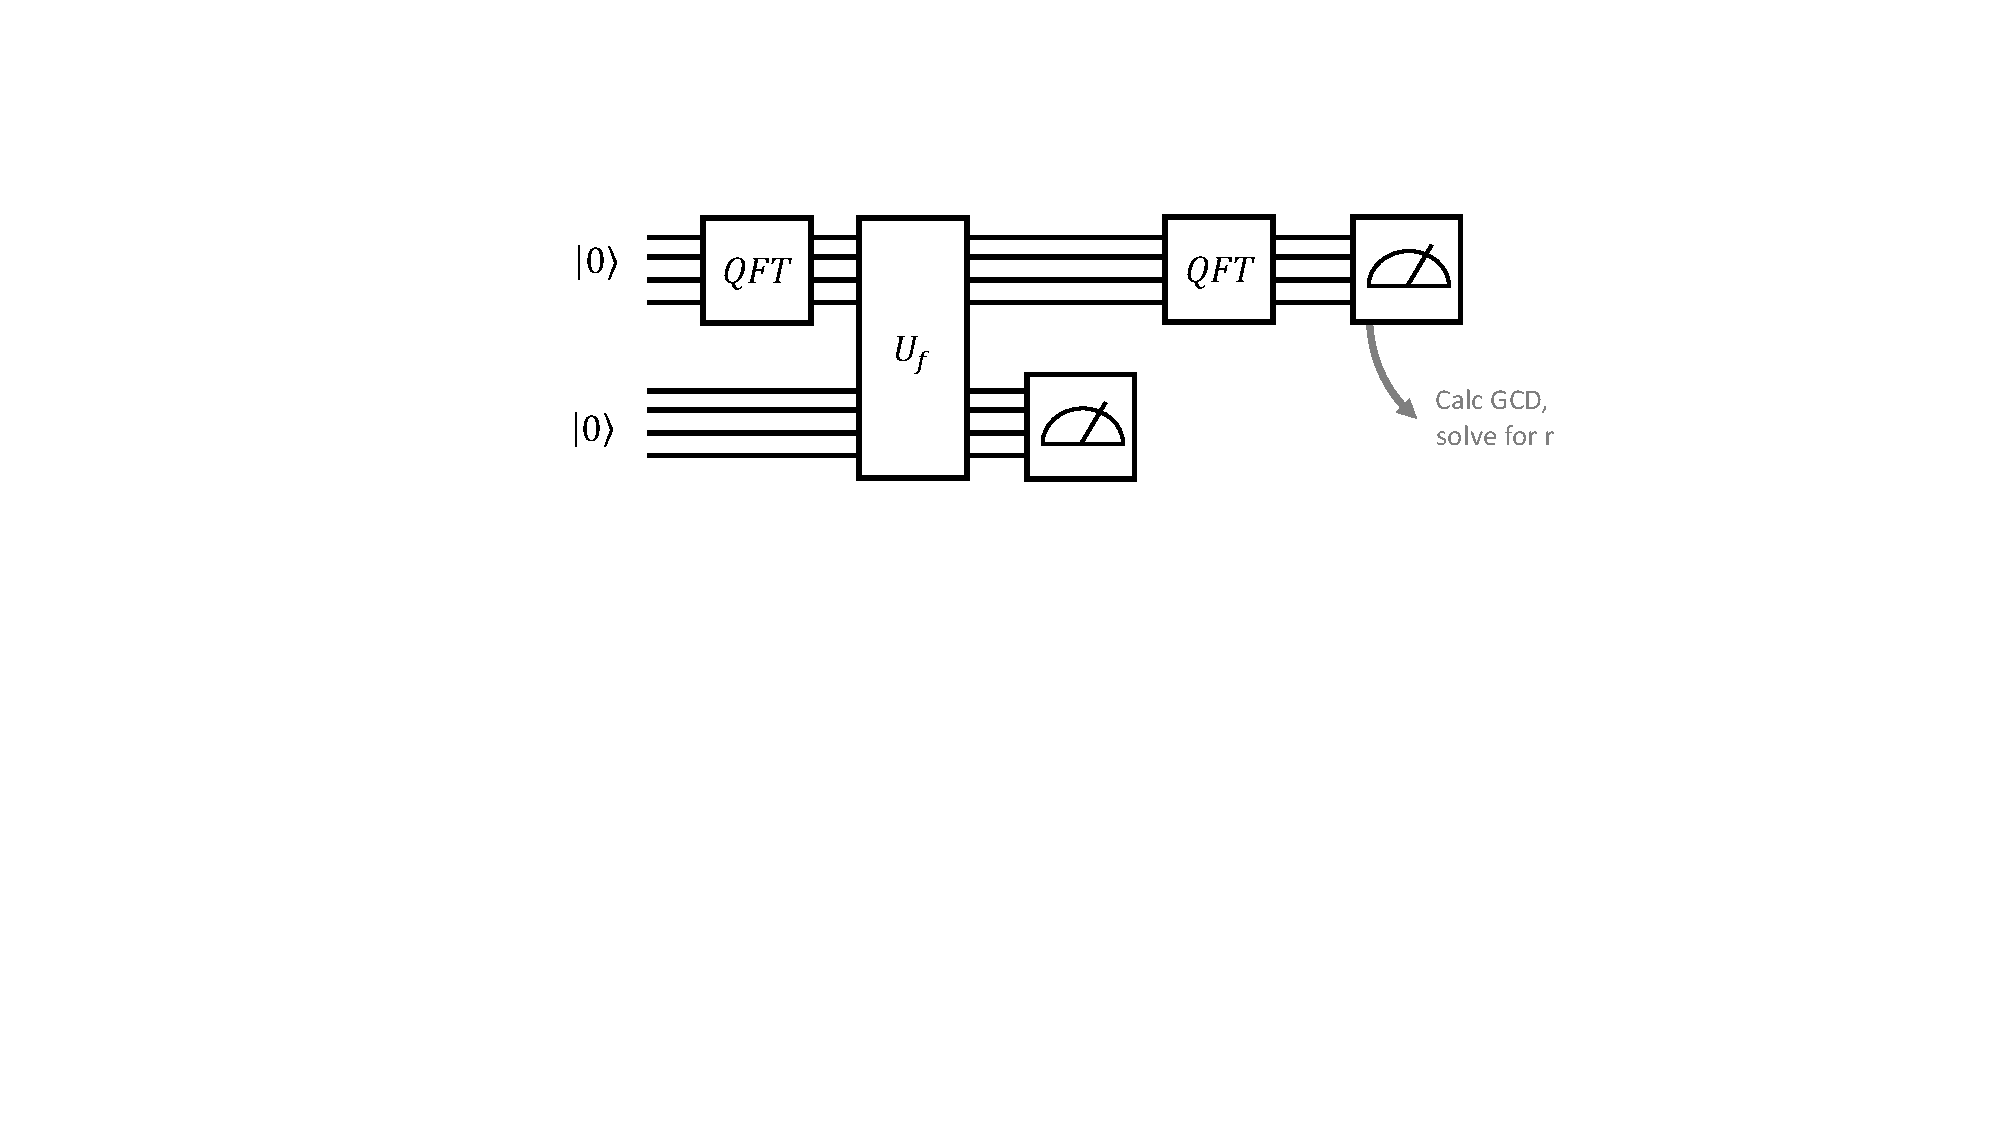
\includegraphics[width=.7\textwidth]{Lecture7Figs/periodfind.pdf}
\end{figure}

\subsection{Modular Arithmetic Review}
In order to apply the problem of period finding to integer factorization, there are few key definitions and lemmas of modular arithmetic that we will need to introduce.
\newline\newline
\underline{Definition}: $x$ is a \textit{non-trivial square root} of $1\pmod N$ if $x^2\equiv 1\pmod N$.
\newline 
ex) 2 is a non-trivial square root of 3: $2^2=4\equiv1 \pmod3$
\newline\newline
\underline{Lemma 1}: Factoring is equivalent to finding the non-trivial square root of $1\pmod N$.
\textit{Proof}:
\begin{equation*}
    x^2-1\equiv 0 \pmod N \quad\Rightarrow\quad x^2-1 \text{ is a multiple of } N 
\end{equation*}
\begin{equation*}
    N | (x+1)(x-1) \quad \text{but}\quad N \nmid (x \pm 1) \quad \text{[ because } x\nequiv \pm 1\pmod N\text{ ]}
\end{equation*}
\centerline{$\gcd(N,x \pm 1)$ are factors of $N$ (can compute using Euclid's algorithm)}
\newline\newline
\underline{Definition}: The \textit{order} of $x\pmod N$ is the smallest integer $r$ such that $x^r \equiv 1\pmod N$.
\newline In other words, the order of $x$ is just the period of $f(i)=x^i\pmod N$.
\newline\newline
\underline{Lemma 2}: Suppose $N=pq$ and $x \neq p,q$, then with probability $\geq \frac{1}{2}$ the order $s$ is even and $x^{\frac{s}{2}}$ is a non-trivial square root of $1 \pmod N$. [Proof requires number theory beyond the scope of this class.]

\subsection{Shor's Algorithm}
In order to factor the number $N$ using Shor's algorithm, we will need $m$ qubits such that $2^m >> N^2$ (since the order of random numbers might be as large as $N$). Using Lemmas 1 and 2, Shor's algorithm can be reduced to the following 3 steps,
\begin{enumerate}
    \item Pick a random number.
    \item Use the period finding algorithm to find its order.
    \item If the order is even, find the non-trivial square root. If the order is odd or $x^{\frac{s}{2}}=-1$, start over from Step 1.
\end{enumerate}
Because of Lemma 2, we can be confident that we will factor $N$ in just a few runs of the algorithm. Since this is primarily an application of period finding, the circuit looks very similar to the period finding circuit.

\subsection{Example}
We now go through an example of the integer factorization procedure for the quantity 119. 
\newline\newline
\underline{Step 1}: Guess 16.
\newline\newline
\underline{Step 2}: Find the order:
\begin{enumerate}
    \item $16\equiv 16\pmod{119}$
    \item $16\times16=256\equiv18$
    \item $18\times16=288\equiv50$
    \item $50\times16=800\equiv86$
    \item $86\times16=1376\equiv67$
    \item $67\times16=1072=119\times17+1\equiv1$
\end{enumerate}
Thus, the order of $16\pmod{119}$ is 6.
\newline\newline
\underline{Step 3}: Compute $16^3\equiv 50$:
\begin{equation*}
    \begin{rcases}
        \gcd(49,119)=7 \\
        \gcd(51,119)=17 \quad
    \end{rcases}
    \quad7\times17=119
\end{equation*}

\section{Grover's Algorithm}
Following Shor's algorithm, in 1995, Lov Grover proposed the quantum search algorithm now known as Grover's algorithm. Although Grover's algorithm did not provide as spectacular of a speedup (exponential) as Shor's algorithm, the widespread applicability of search-based methodologies created considerable interest in it. 
\newline
\newline
As we will see, classical linear search requires $O(N)$ operations, while quantum search requires $O(\sqrt{N})$ operations. Note that while faster classical search algorithms exist (i.e. binary search is $O(\log(n))<O(\sqrt{N})$), but these algorithms require a \textit{sorted} list of input. If the sorting time is considered, the classical search is overall less efficient.

\subsection{Problem Statement}
Grover's algorithm aims to solve the following problem:
\newline
\newline
\textit{Given a search space of size N, and no prior knowledge about the structure of information in it (i.e. unstructured), find an element of that search space satisfying a known property.}
\newline
\newline
\underline{Given}: a list of $N$ items
\begin{figure}[h!]
    \centering
    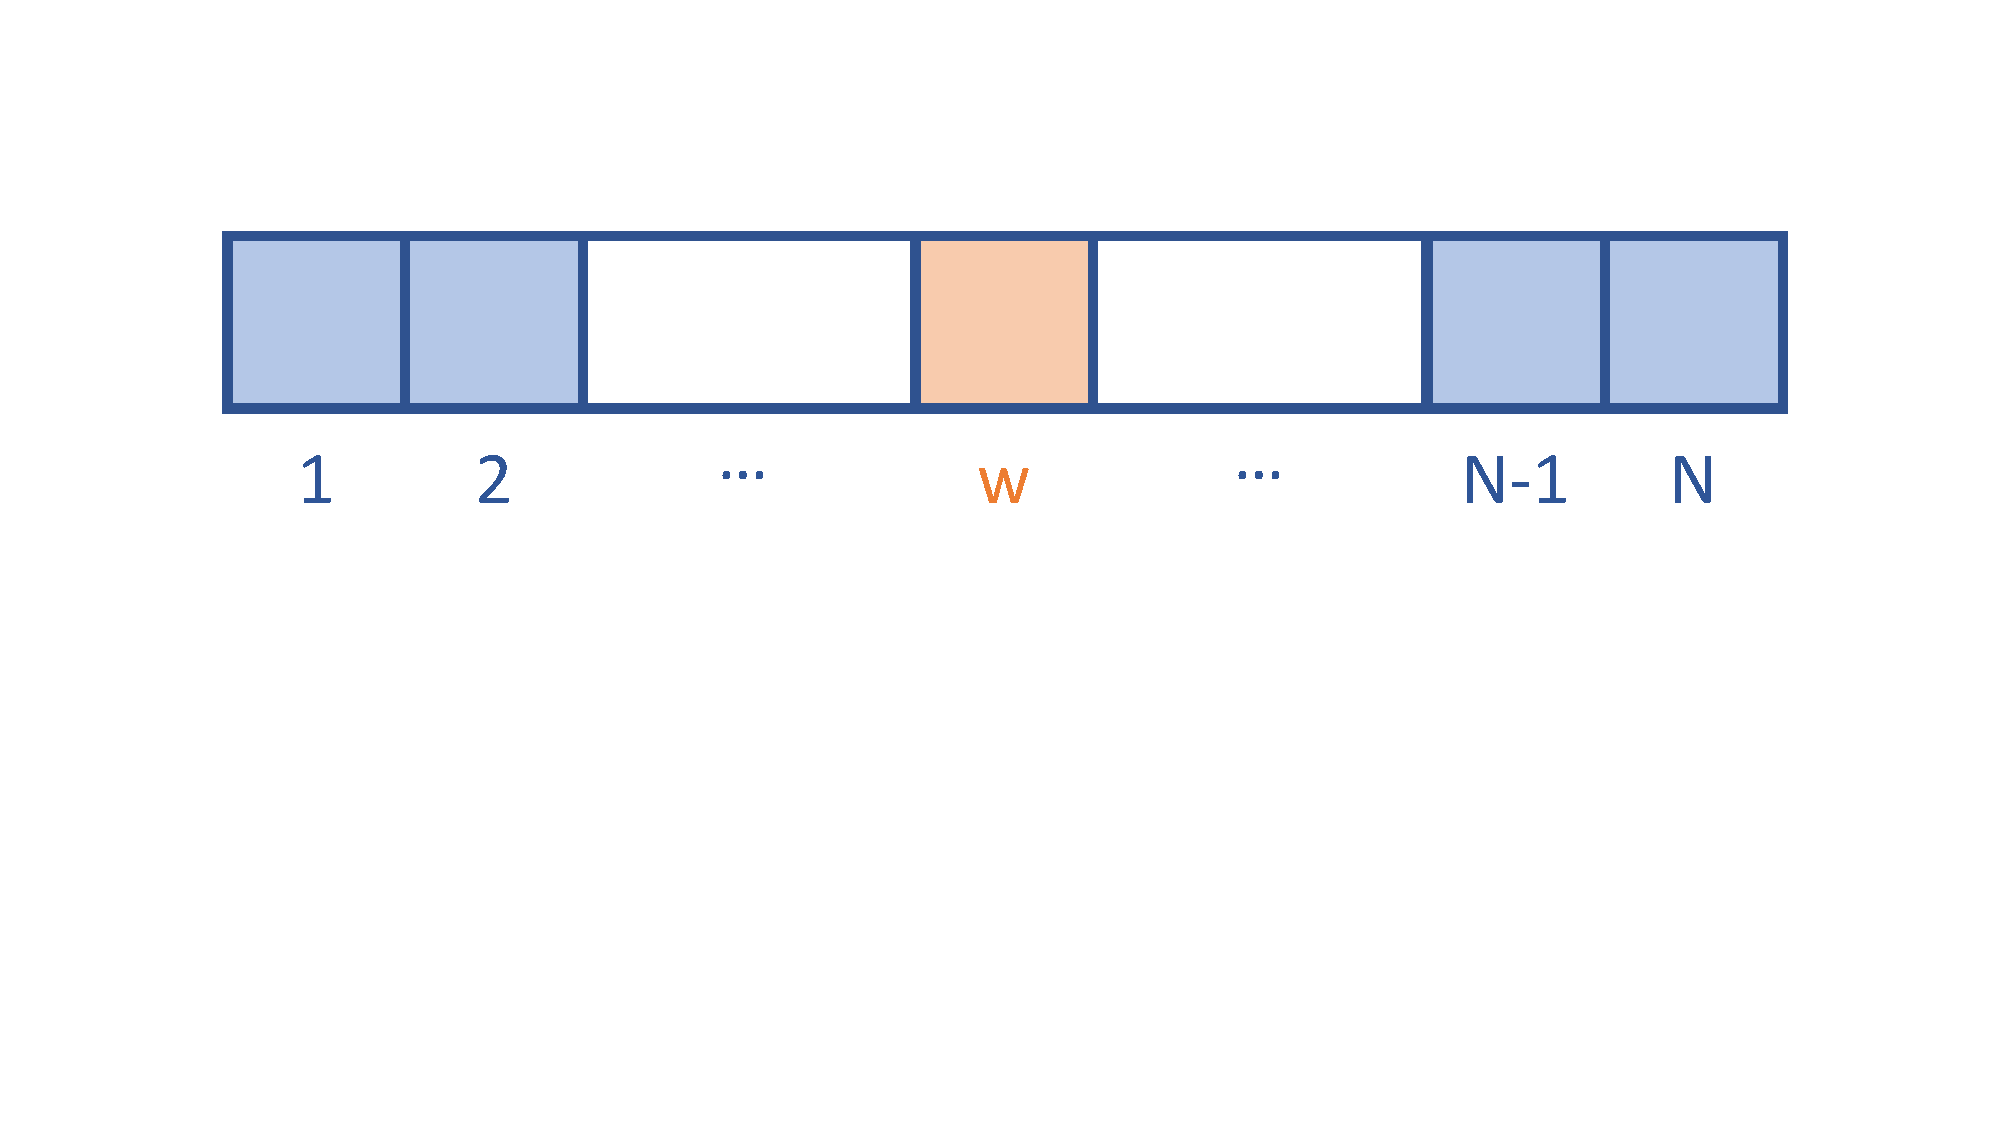
\includegraphics[width=.7\textwidth]{Lecture7Figs/search_items.pdf}
    \label{fig:search_item}
\end{figure}

\noindent\underline{Goal}: identify the winner state ($w$)

\subsection{Mapping to the Quantum Domain}

\noindent \textbf{Q:} How will the list be defined in our quantum computer?
\newline
\noindent \textbf{A:} With an \underline{oracle}.
\newline
\newline
In this case, the oracle is a ``black-box" function which returns 0 for unmarked input and 1 for the winner input
\[
    f(x)= 
\begin{cases}
    1, & \text{if } x=w\\
    0, & \text{if } x\neq w
\end{cases}
\]
In the quantum computer the oracle will be encoded as a \textit{unitary matrix} and the list of items will be provided as a \textit{superposition} of states. In order to 
represent the list items with qubits, we must choose a binary encoding $x,w \in {0,1}^n$ such that $N=2^n$ (where $n$ is the number of list items).
\newline
\newline
\textit{Example}: Suppose we have a list of length $N=8$, we need 3-bit binary encodings (8=2$^3$).
\centerline{$|000\rangle$, $|001\rangle$, $|010\rangle$, $|011\rangle$, $|100\rangle$, $|101\rangle$, $|110\rangle$, $|111\rangle$}
\newline
\newline
\underline{Important Note}: You may be wondering what the point of the oracle is at this point...It seems as though the oracle already knows the answer to the search problem?! However, a distinction should be made. You can \textit{recognize} the solution to a search problem without actually \textit{knowing} the solution. The power of the quantum computer lies in out ability to apply this recognition function to \textit{all} $N$ items at once (with superposition), rather than testing each item individually, as is done classically.
\newline
\newline
We define the Grover oracle as unitary matrix $U_f$, which acts on any of the standard basis states $|x\rangle$ by,
\begin{equation*}
    U_f|x\rangle=(-1)^{f(x)}|x\rangle.
\end{equation*}
If $x$ is unmarked, the oracle does nothing to the state. If $x$ is a winner state, then $U_f|x\rangle=U_f|w\rangle=-|w\rangle$.
\newline
\newline
Now, all that is left is to define the input state to our system. Before looking at our list of items, we have no idea where the winner state is. Any guess of its location is as good as any other, meaning our input should be a \textit{uniform} superposition state,
\begin{equation*}
    |s\rangle = \frac{1}{\sqrt{N}}\sum_{x=0}^{N-1}|x\rangle.
\end{equation*}
If we were to stop here and measure our state, the superposition would collapse to any one of the basis states with the \textit{same} probability, $\frac{1}{N}=\frac{1}{2^n}$.

\subsection{Geometric Picture}
Grover's algorithm uses a procedure called \textit{amplitude amplification} to significantly enhance the probability of measuring the winner state. Geometrically, we can picture the 2 special states (winner $|w\rangle$ and $|s\rangle$) as 2 vectors spanning $\mathbb{C}^N$.
\begin{figure}[h!]
    \centering
    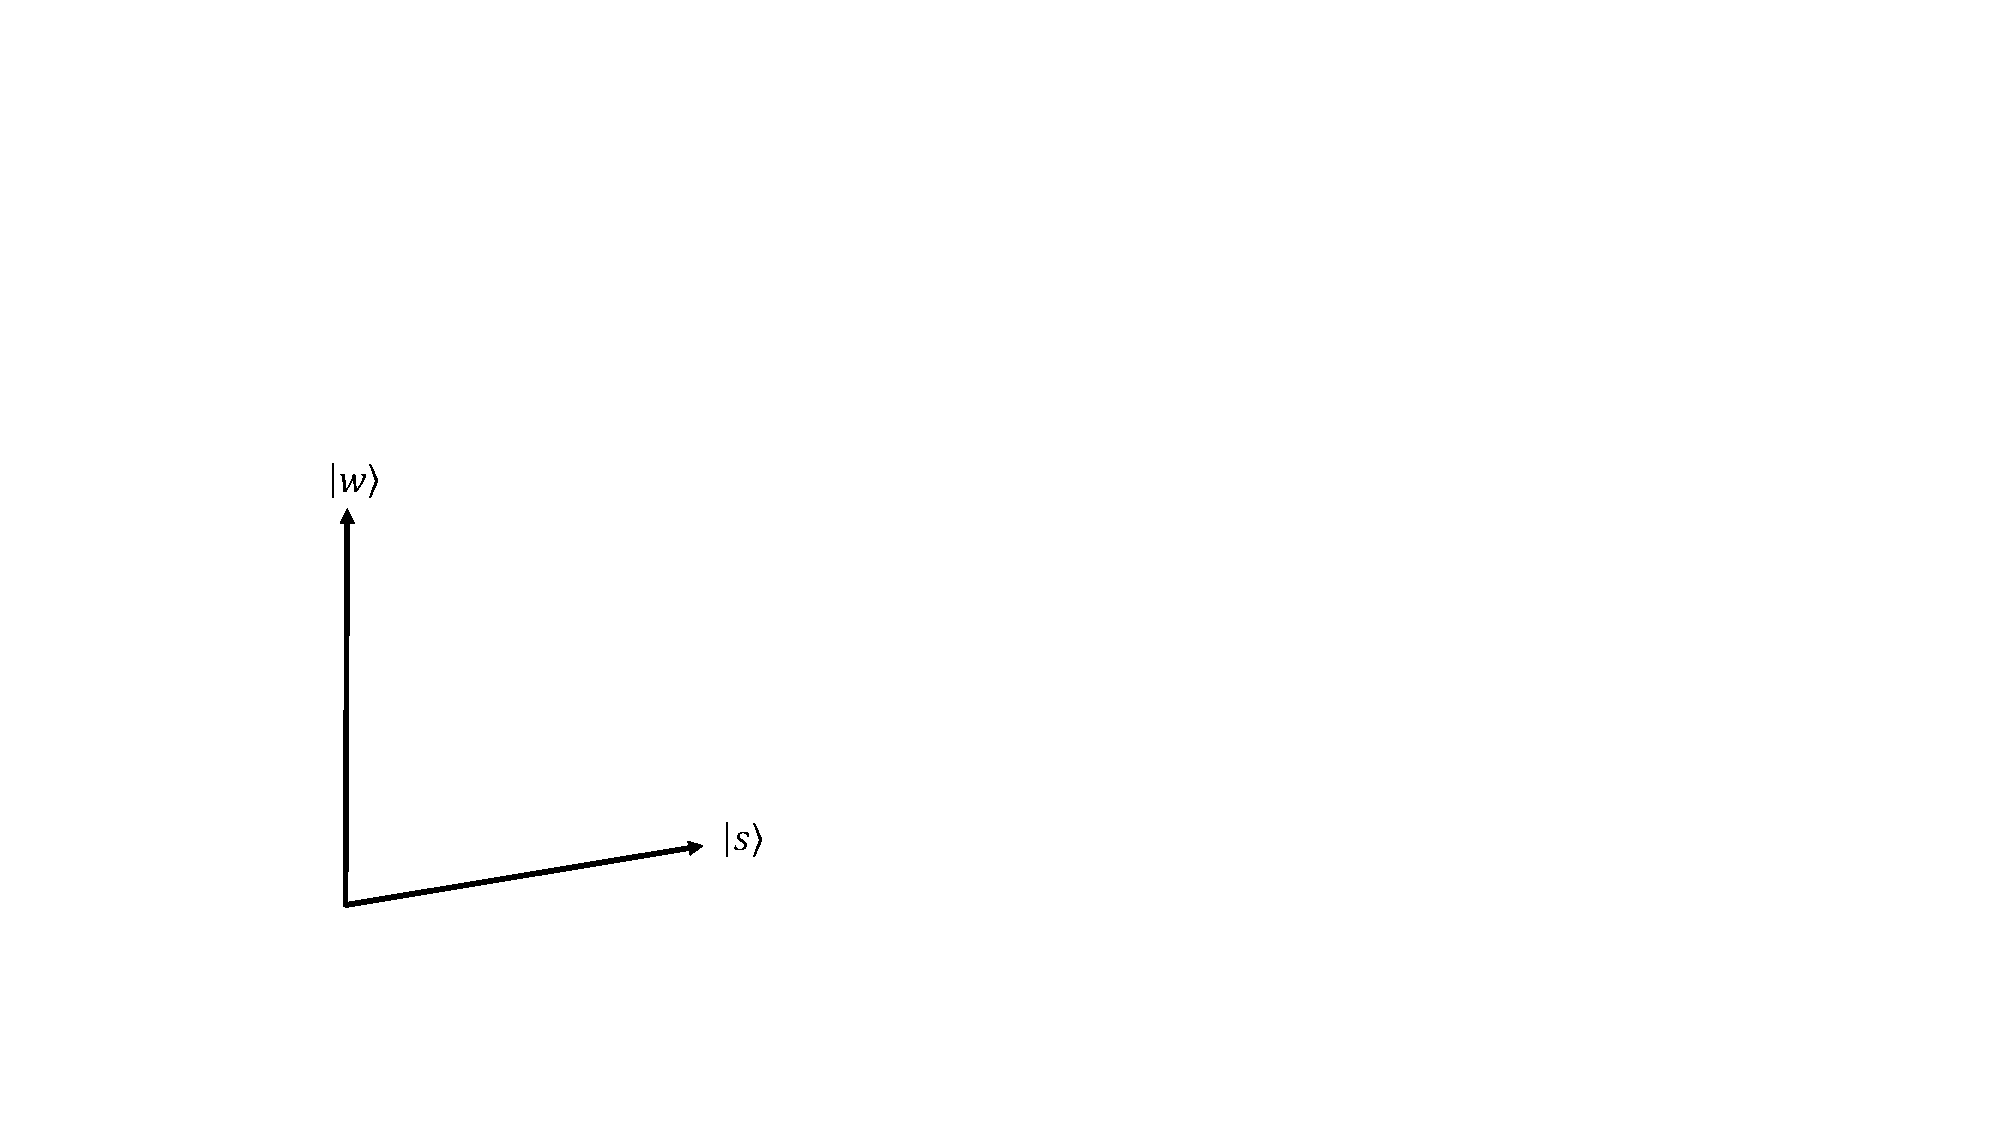
\includegraphics[width=.3\textwidth]{Lecture7Figs/sw.pdf}
    \label{fig:search_item}
\end{figure}
\newline
However, since $|s\rangle$, is a superposition over all possible states (including $|w\rangle$), it is not perpendicular to $|s\rangle$. Thus, we introduce orthogonal state $|s'\rangle$.
\begin{figure}[h!]
    \centering
    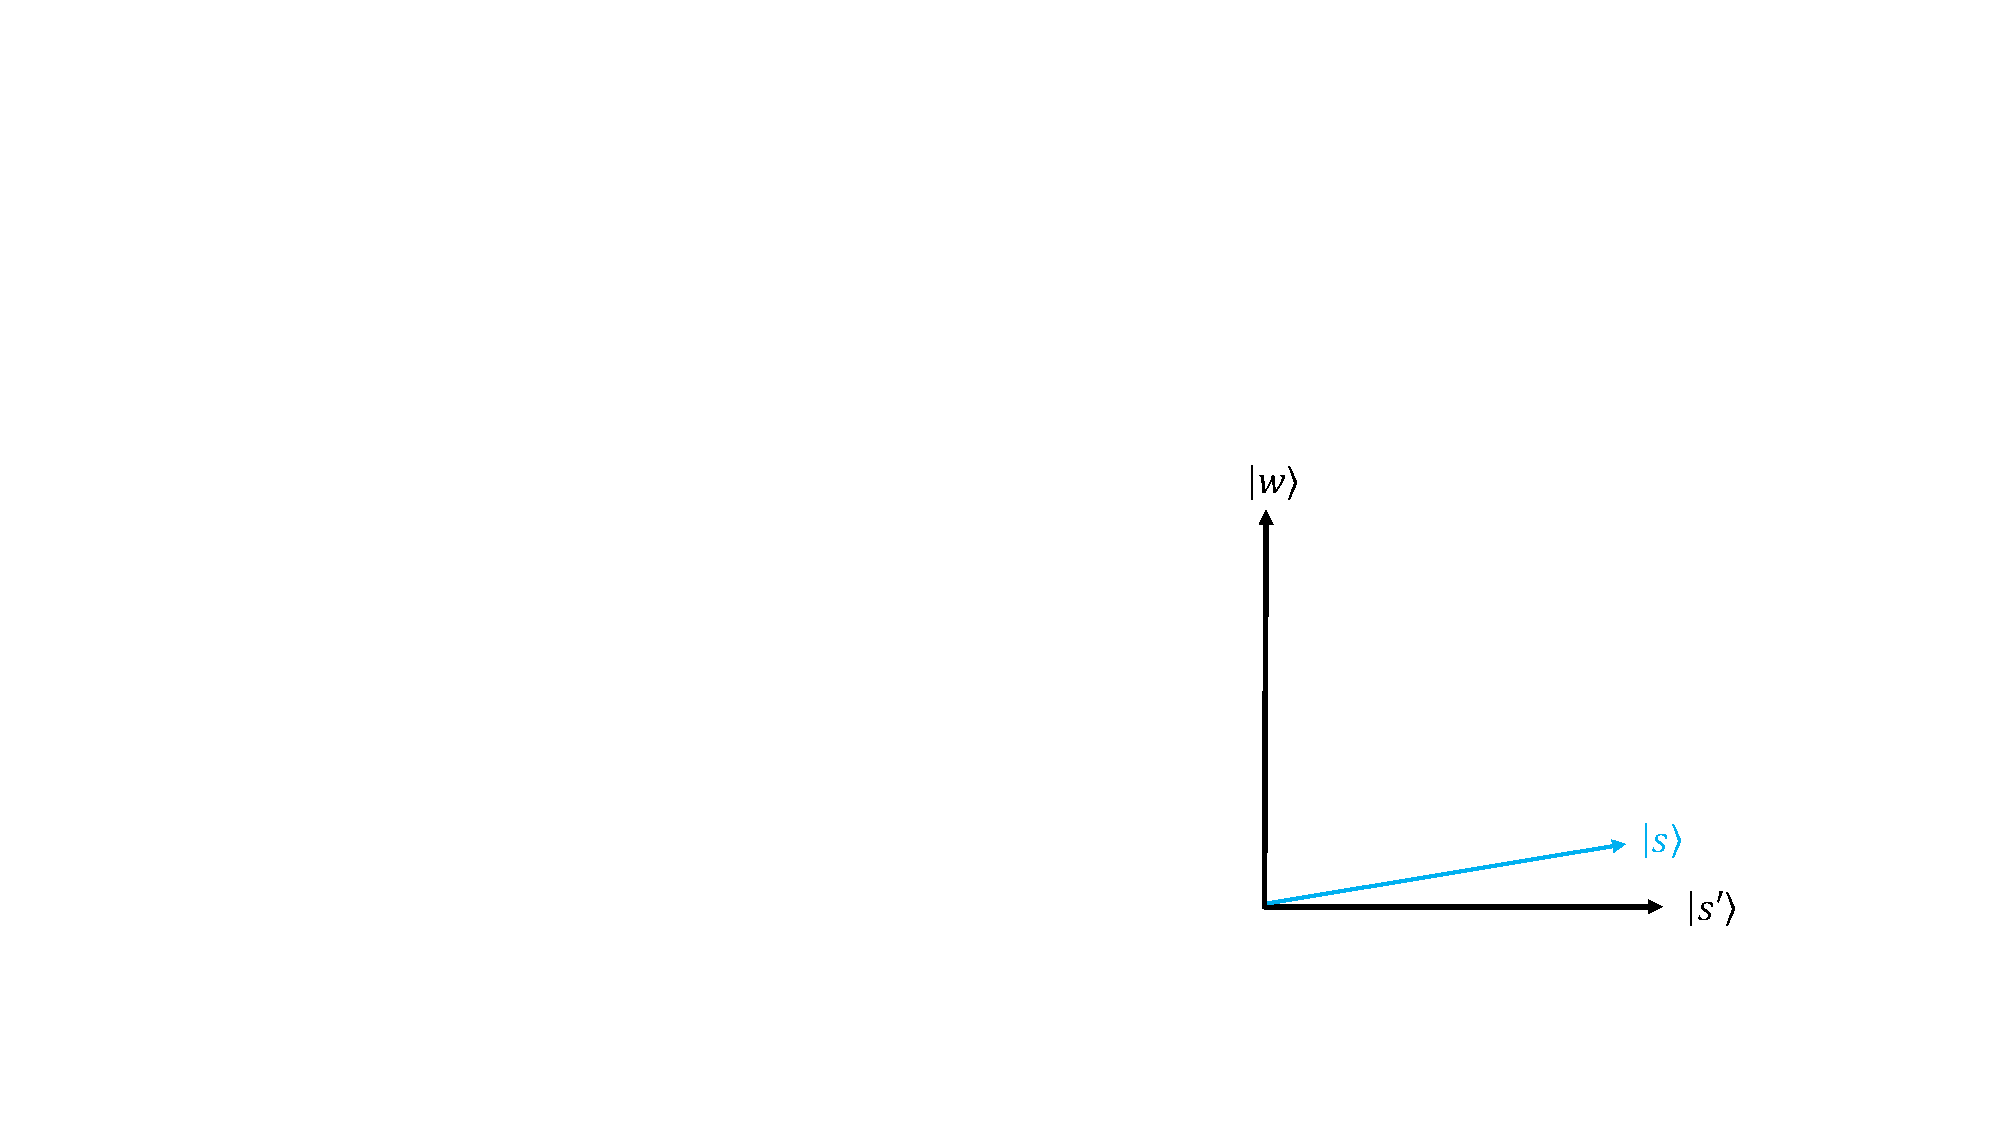
\includegraphics[width=.3\textwidth]{Lecture7Figs/ss'w.pdf}
    \label{fig:search_item}
\end{figure}
$|s'\rangle$ is obtained from $|s\rangle$ by removing $|w\rangle$ and rescaling (as in the Gram-Schmidt process).

\subsection{Amplitude Amplification Procedure}
We now have everything we need to describe the procedure of Grover's algorithm!
\newline
\newline
\underline{Step 0: Initialization}
\newline
Initialize to superposition state, at $t=0$, 
\begin{equation*}
    |\Psi_0\rangle=|s\rangle=H^{\otimes n}|0\rangle^n \qquad \Bigg(=\frac{1}{\sqrt{N}}\sum_{x=0}^{N-1}|x\rangle\Bigg)
\end{equation*}
The average amplitude of $N$ states is $\frac{1}{\sqrt{N}}$.
\begin{figure}[h!]
    \centering
    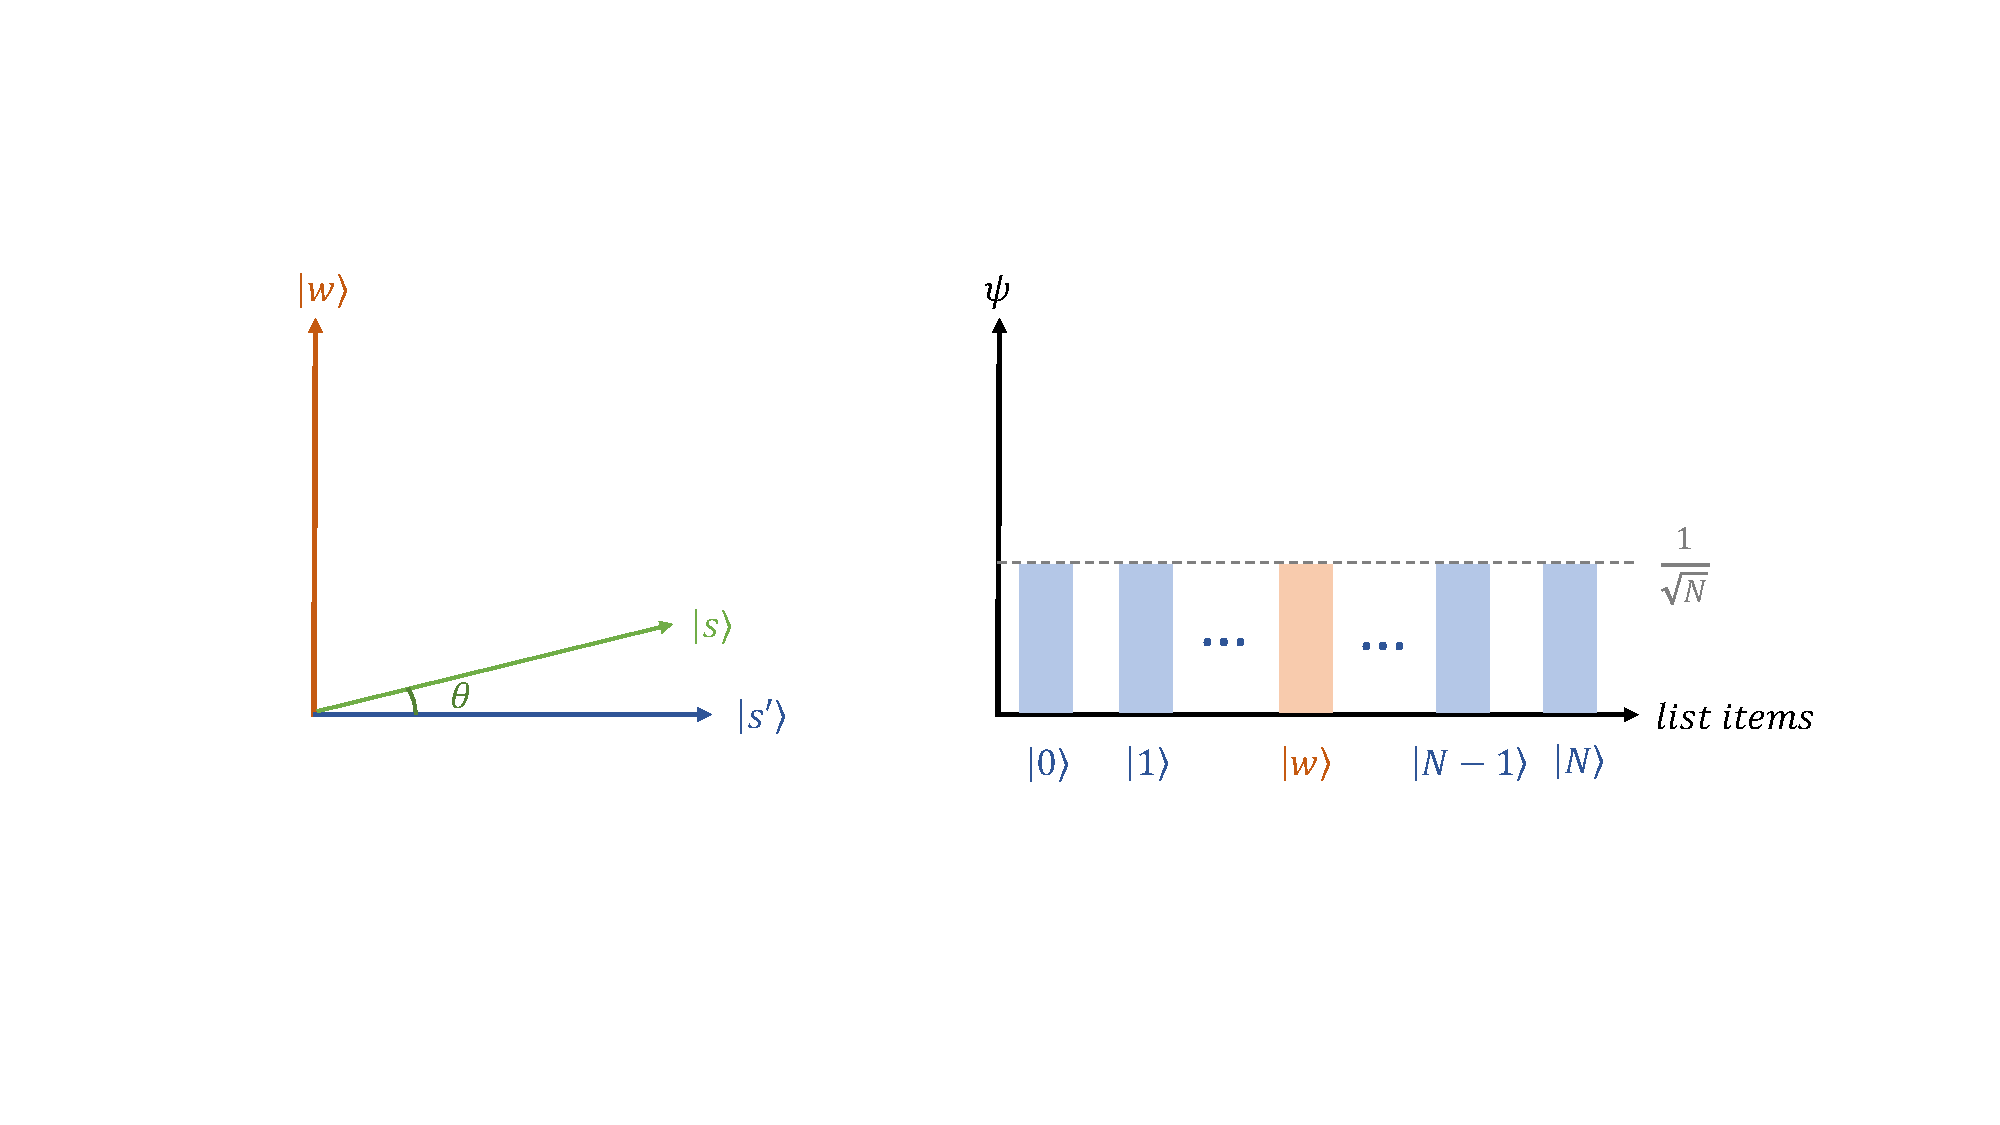
\includegraphics[width=.95\textwidth]{Lecture7Figs/step1.pdf}
    \label{fig:search_item}
\end{figure}
\newpage
\noindent\underline{Step 1: Apply Oracle}
\newline
Apply the oracle, $U_f$,
\begin{equation*}
    |\Psi_{t'}\rangle = U_f |\Psi_0\rangle.
\end{equation*}
Geometrically, $U_f$ corresponds to a reflection of state $|\Psi_0\rangle$ about $|s'\rangle$. Thus, the amplitude of the $|w\rangle$ state becomes negative and the overall average amplitude is lowered \big($<\frac{1}{\sqrt{N}}$\big).
\begin{figure}[h!]
    \centering
    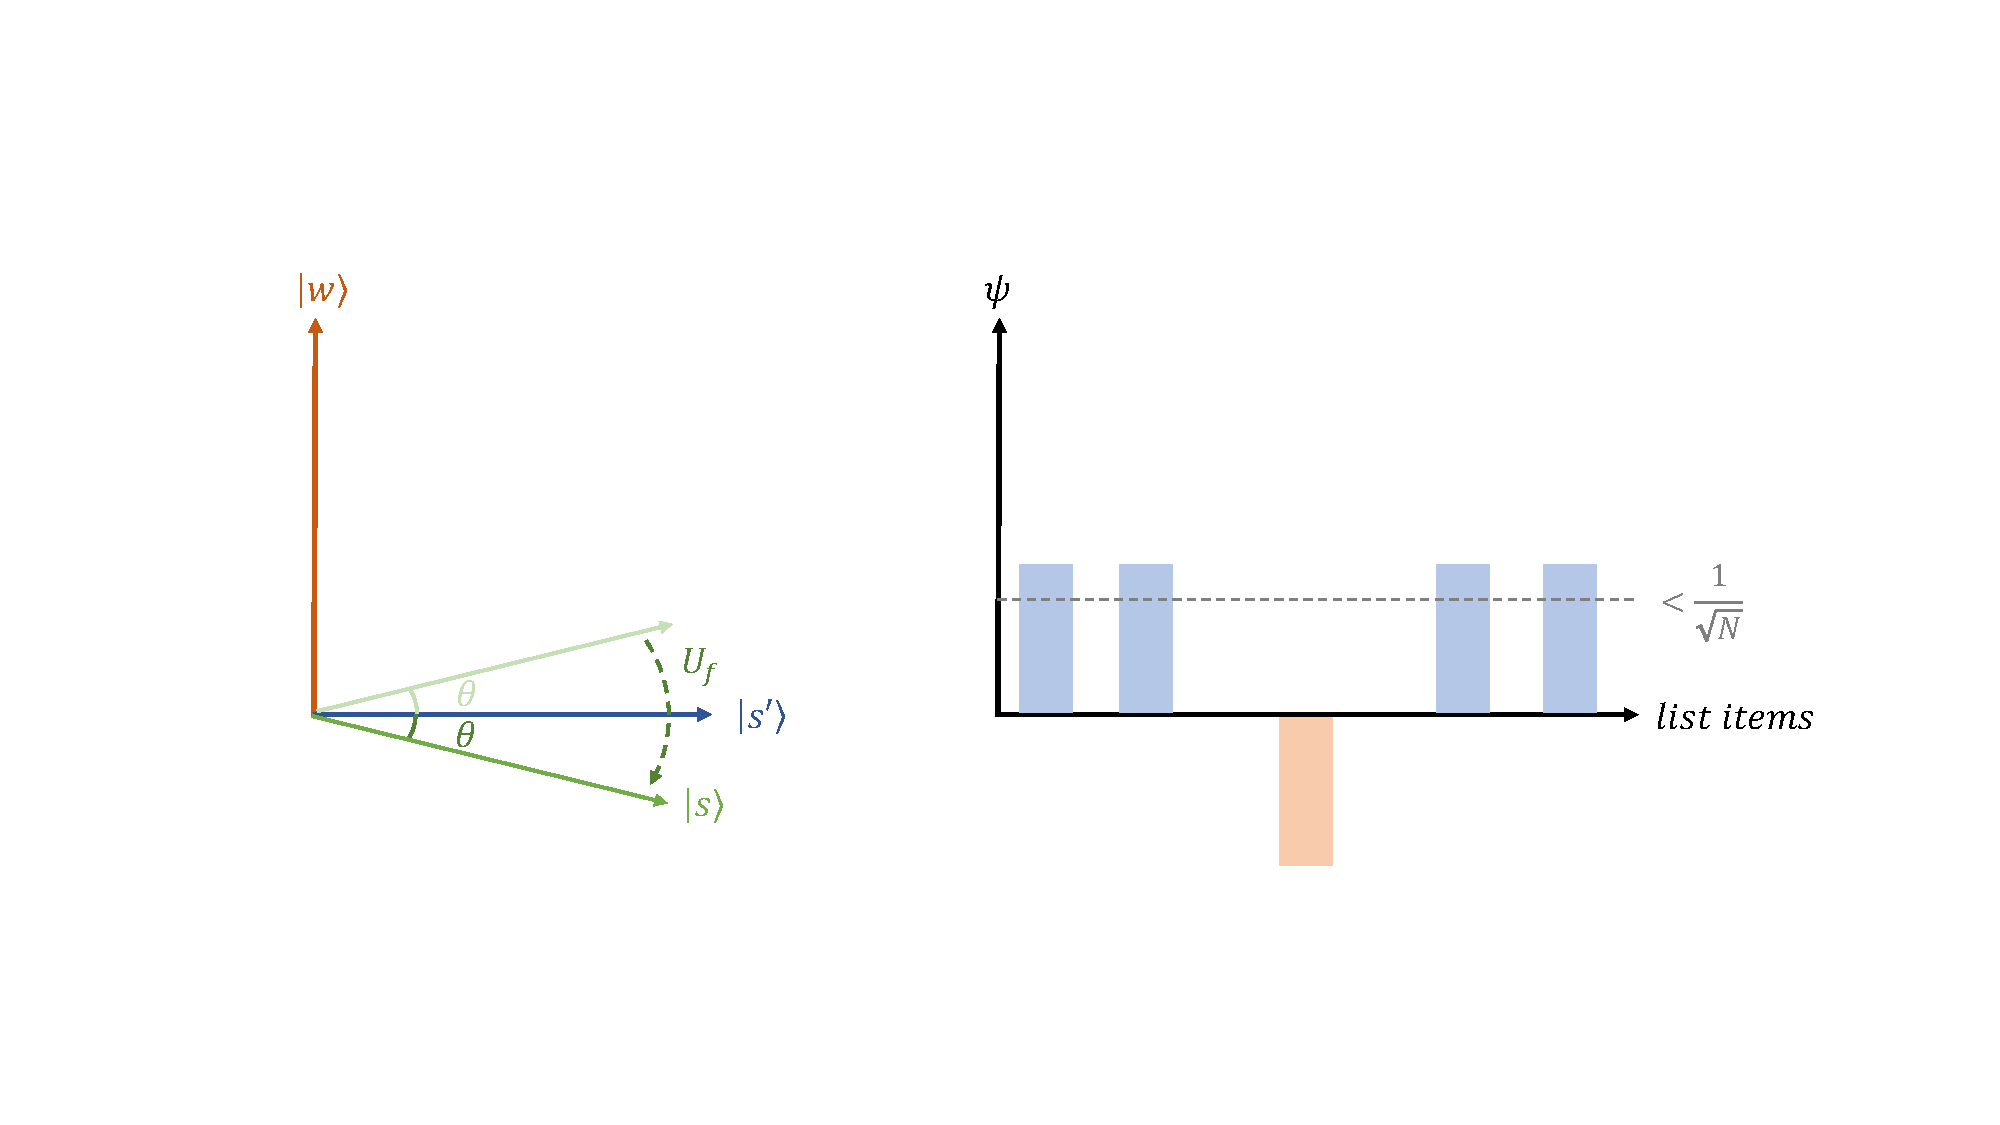
\includegraphics[width=.95\textwidth]{Lecture7Figs/step2.pdf}
    \label{fig:search_item}
\end{figure}
\newline
\underline{Step 2: Amplitude Amplification}
\newline
Apply $U_s=2|s\rangle\langle s|-\mathbb{I}$,
\begin{equation*}
     |\Psi_{t}\rangle = U_s |\Psi_{t'}\rangle = U_s U_f |\Psi_0\rangle.
\end{equation*}
Geometrically, $U_s$ corresponds to a reflection of state $|\Psi_{t'}\rangle$ about $|s\rangle$. From the perspective our measurement amplitudes, this corresponds to a reflection about the average amplitude. 
\begin{figure}[h!]
    \centering
    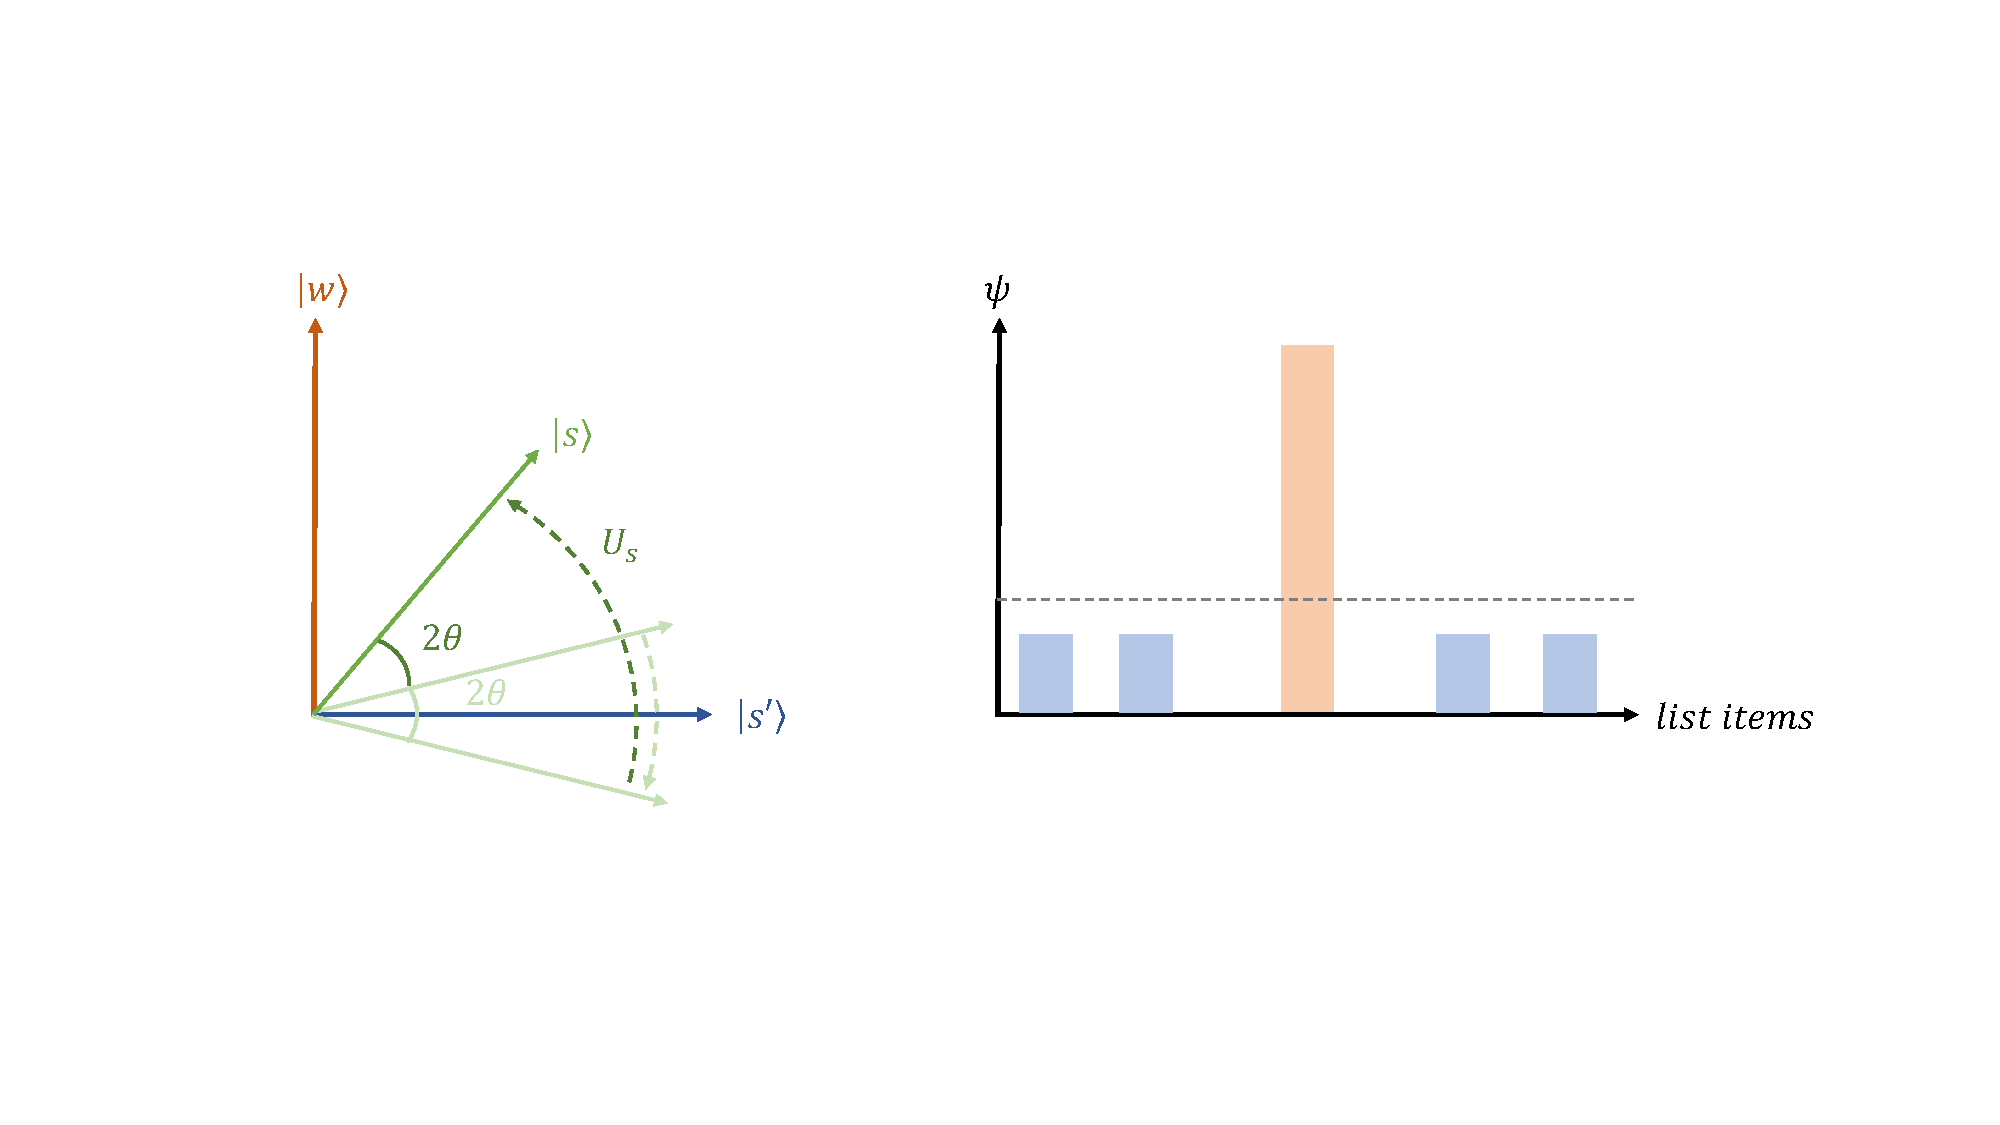
\includegraphics[width=.95\textwidth]{Lecture7Figs/step3.pdf}
    \label{fig:search_item}
\end{figure}
We can verify this mathematically by applying the operation $(2|s\rangle\langle s|-\mathbb{I})$, with $|s\rangle = \frac{1}{\sqrt{N}}\sum_{x=0}^{N-1}|x\rangle$, to a general state, $\sum_{k=0}^{N-1} \alpha_k |k\rangle$, with average $\langle\alpha\rangle=\sum_k \alpha_k|\langle s|k\rangle|^2$,
\begin{equation*}
    \begin{array} {lcl} 
        (2|s\rangle\langle s|-\mathbb{I}) \sum_k \alpha_k |k\rangle & = & \sum_k 2\alpha_k |s\rangle\langle s|k\rangle-\alpha_k |k\rangle \\[5pt] 
        & = & \sum_k 2\alpha_k |s\rangle \bigg(\frac{1}{\sqrt{N}}\sum_x\langle x|k\rangle\bigg)-\alpha_k |k\rangle \\[10pt]
        & = & \sum_k 2\alpha_k |s\rangle \bigg(\frac{1}{\sqrt{N}}\sum_x\delta_{xk}\bigg)-\alpha_k |k\rangle \\[10pt]
        & = & \sum_k \frac{2\alpha_k}{\sqrt{N}} |s\rangle-\alpha_k |k\rangle \\[10pt]
        & = & \sum_k \frac{2\alpha_k}{\sqrt{N}} \bigg(\frac{1}{\sqrt{N}}\sum_x|x\rangle\bigg)-\alpha_k |k\rangle \\[15pt]
        & = & 2\sum_k \sum_x\frac{\alpha_k}{N}|x\rangle-\sum_k\alpha_k |k\rangle \\[10pt]
        & = & 2\sum_x\big(\sum_k \alpha_k|\langle s|k\rangle|^2\big)|x\rangle-\sum_k\alpha_k |k\rangle \\[10pt]
        & = & \sum_x 2\langle\alpha\rangle |x\rangle-\sum_k\alpha_k |k\rangle \\[10pt]
        & = & \sum_k \big(2\langle\alpha\rangle-\alpha_k\big) |k\rangle \qed
    \end{array}
\end{equation*}
\underline{Step 3: Repeat}
\newline
Repeat Steps 1 and 2 several times in order to rotate $|s\rangle$ closer to $|w\rangle$
and away from $|s'\rangle$. After $t$ rotations, the state becomes,
\begin{equation*}
    |\Psi_t\rangle=(U_sU_f)^t|\Psi_0\rangle
\end{equation*}
As it turns out, $\sqrt{N}$ rotations are necessary, since the amplitude of $|w\rangle$ grows linearly with the number of applications (grows as $\sim t\sqrt{N}$, where $t=\sqrt{N}$ such that $\langle w|s\rangle\approx 1$).

\subsection{Pseudocode}
1) create superposition of n qubits
\begin{equation*}
    \left.
    \begin{aligned}
        &\text{2) apply oracle O} \\
        &\text{3) apply Hadamard transformation } H^{\otimes n} \\
        &\text{4) perform a conditional phase shift on the computer, with every}\qquad\\
        &\quad\text{computational basis state except $|0\rangle$ receiving a phase shift of -1} \\
        & \hspace{1.7in} |x\rangle\rightarrow -(-1)^{\delta_{x,0}}|x\rangle \\
        & \hspace{1in}\text{can be done with operator } 2|0\rangle\langle 0| - \mathbb{I}\\
        &\text{5) apply Hadamard transformation } H^{\otimes n} \\
    \end{aligned}
    \right\}
    \qquad
    \text{Grover Iteration}
\end{equation*}
6) repeat steps 2-5 (Grover Iteration) $O(\sqrt{N})$ times
\subsection{General Quantum Circuit}
\begin{figure}[h!]
    \centering
    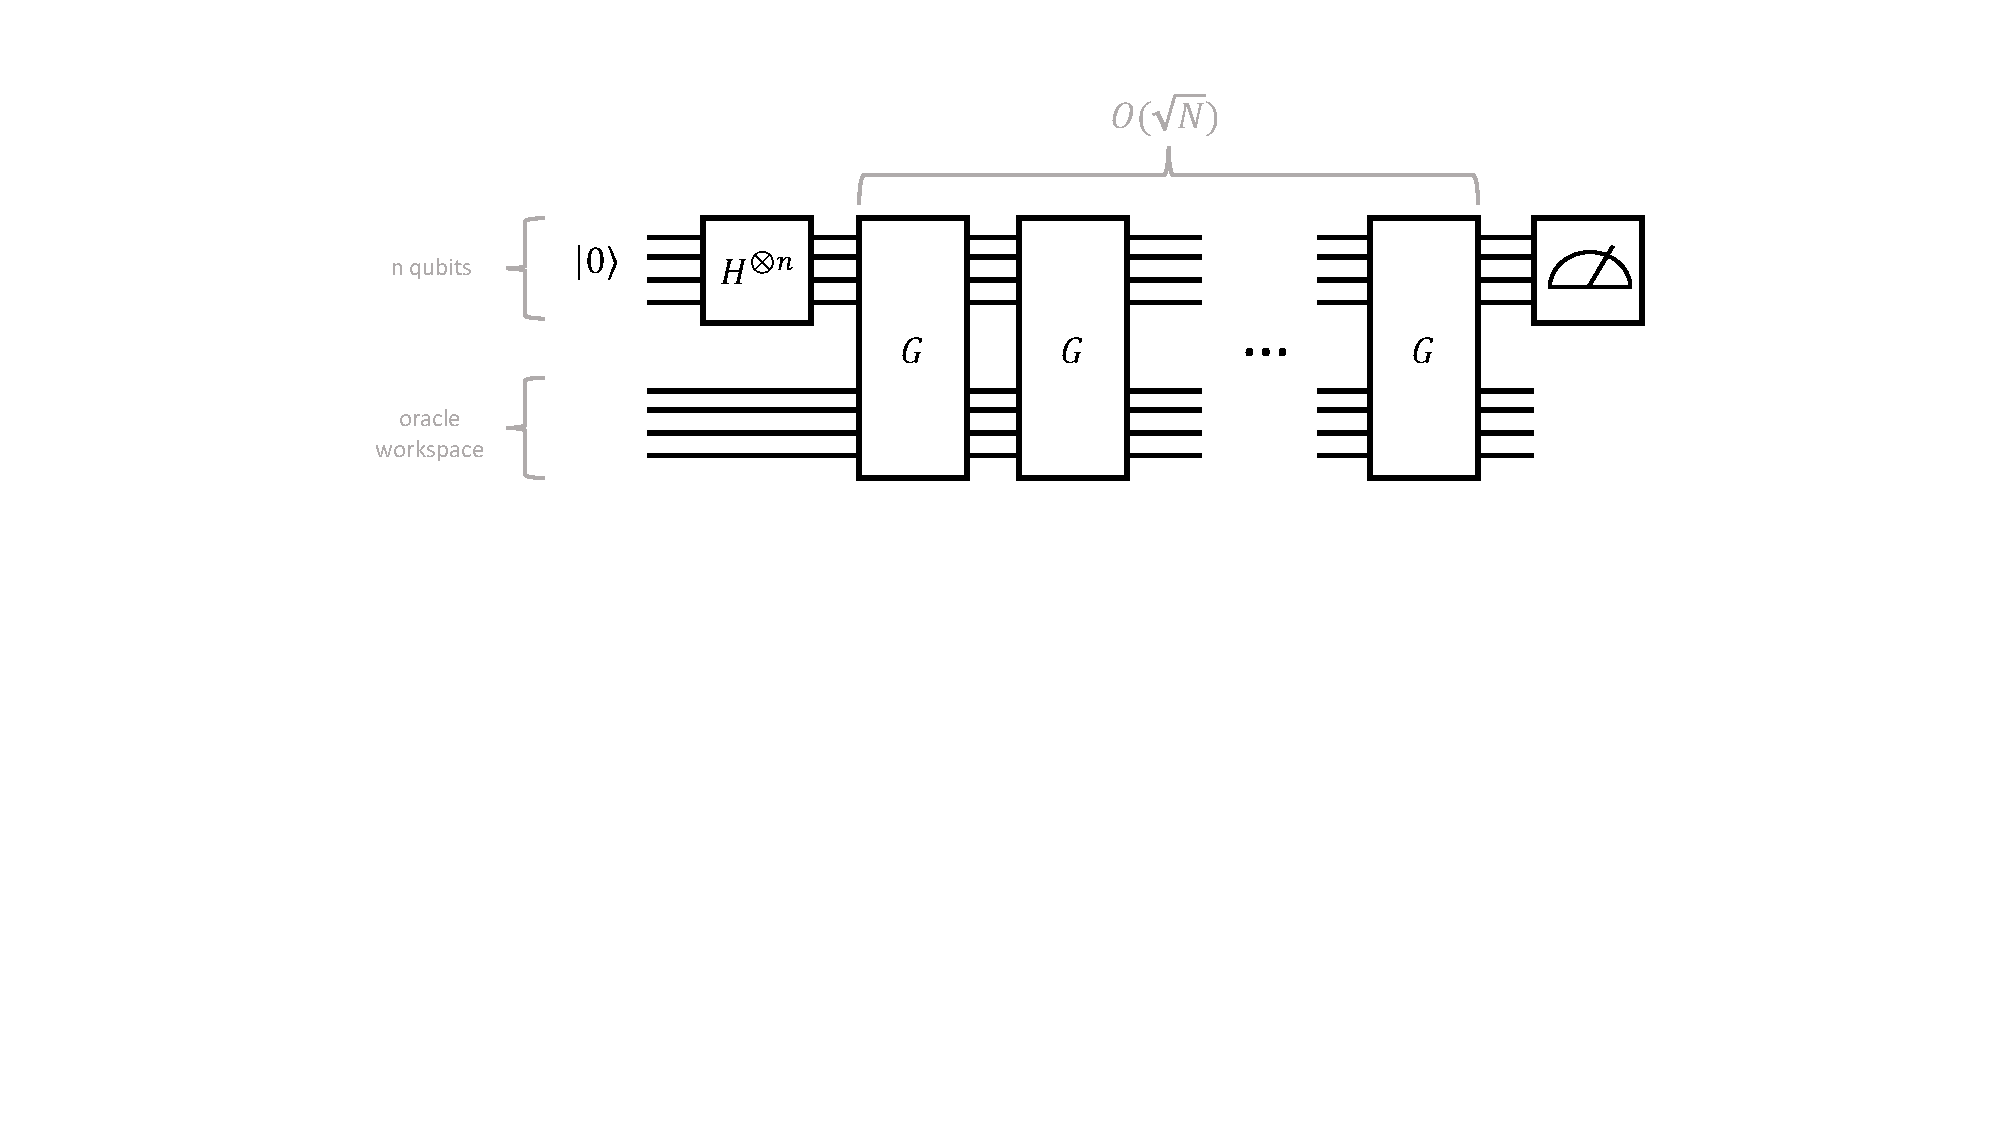
\includegraphics[width=.97\textwidth]{Lecture7Figs/gcircuit.pdf}
    \caption*{Grover search algorithm implementation, where each "G" gate corresponds to a single Grover iteration.}
    \label{fig:search_item}
\end{figure}
\begin{figure}[h!]
    \centering
    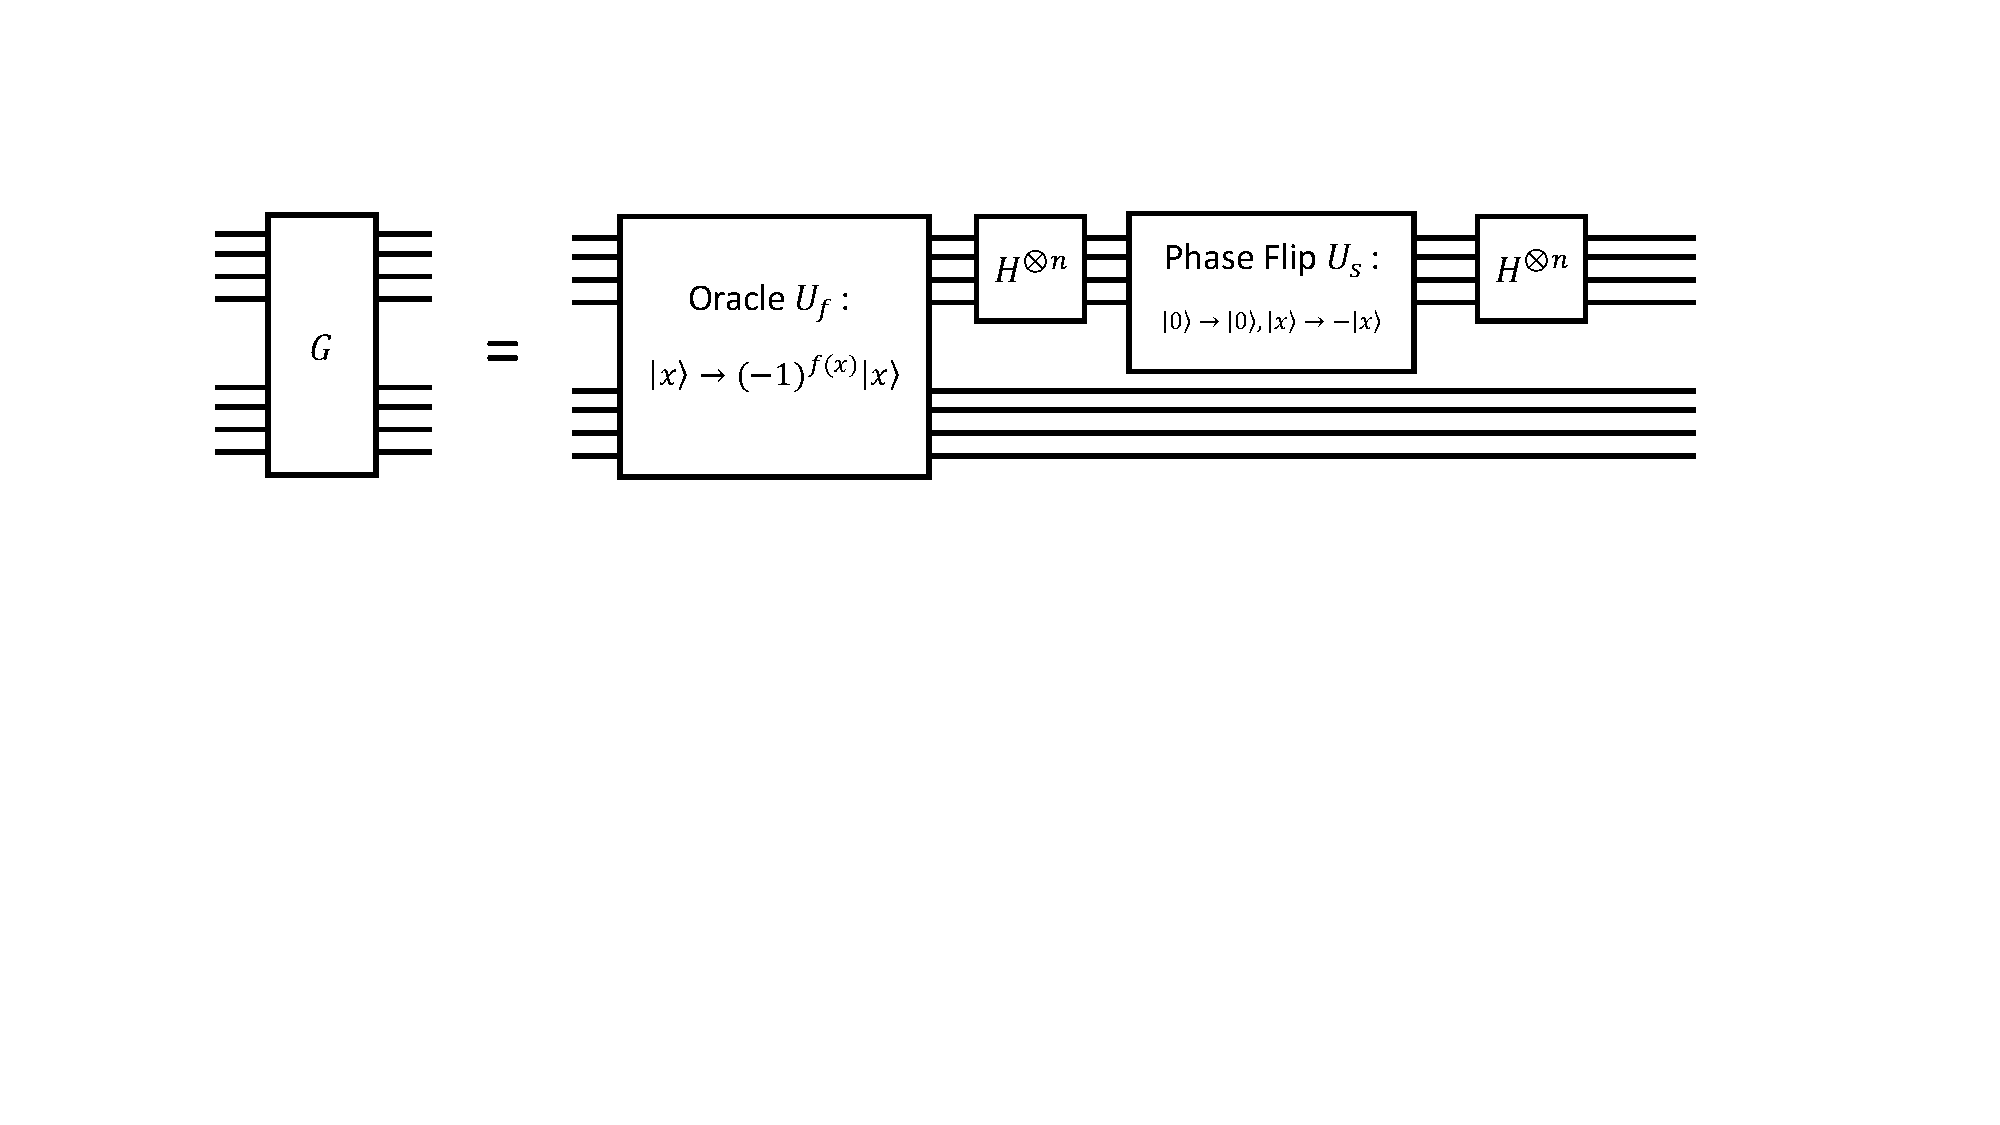
\includegraphics[width=.97\textwidth]{Lecture7Figs/giter.pdf}
    \label{fig:search_item}
\end{figure}

\newpage
\subsection{$N=4$ (2-bit) Implementation Example}
We now provide an example of the exact gates necessary to implement Grover's algorithm to search in a list of 4 items ($|00\rangle$, $|01\rangle$, $|10\rangle$, $|11\rangle$).
\begin{figure}[h!]
    \centering
    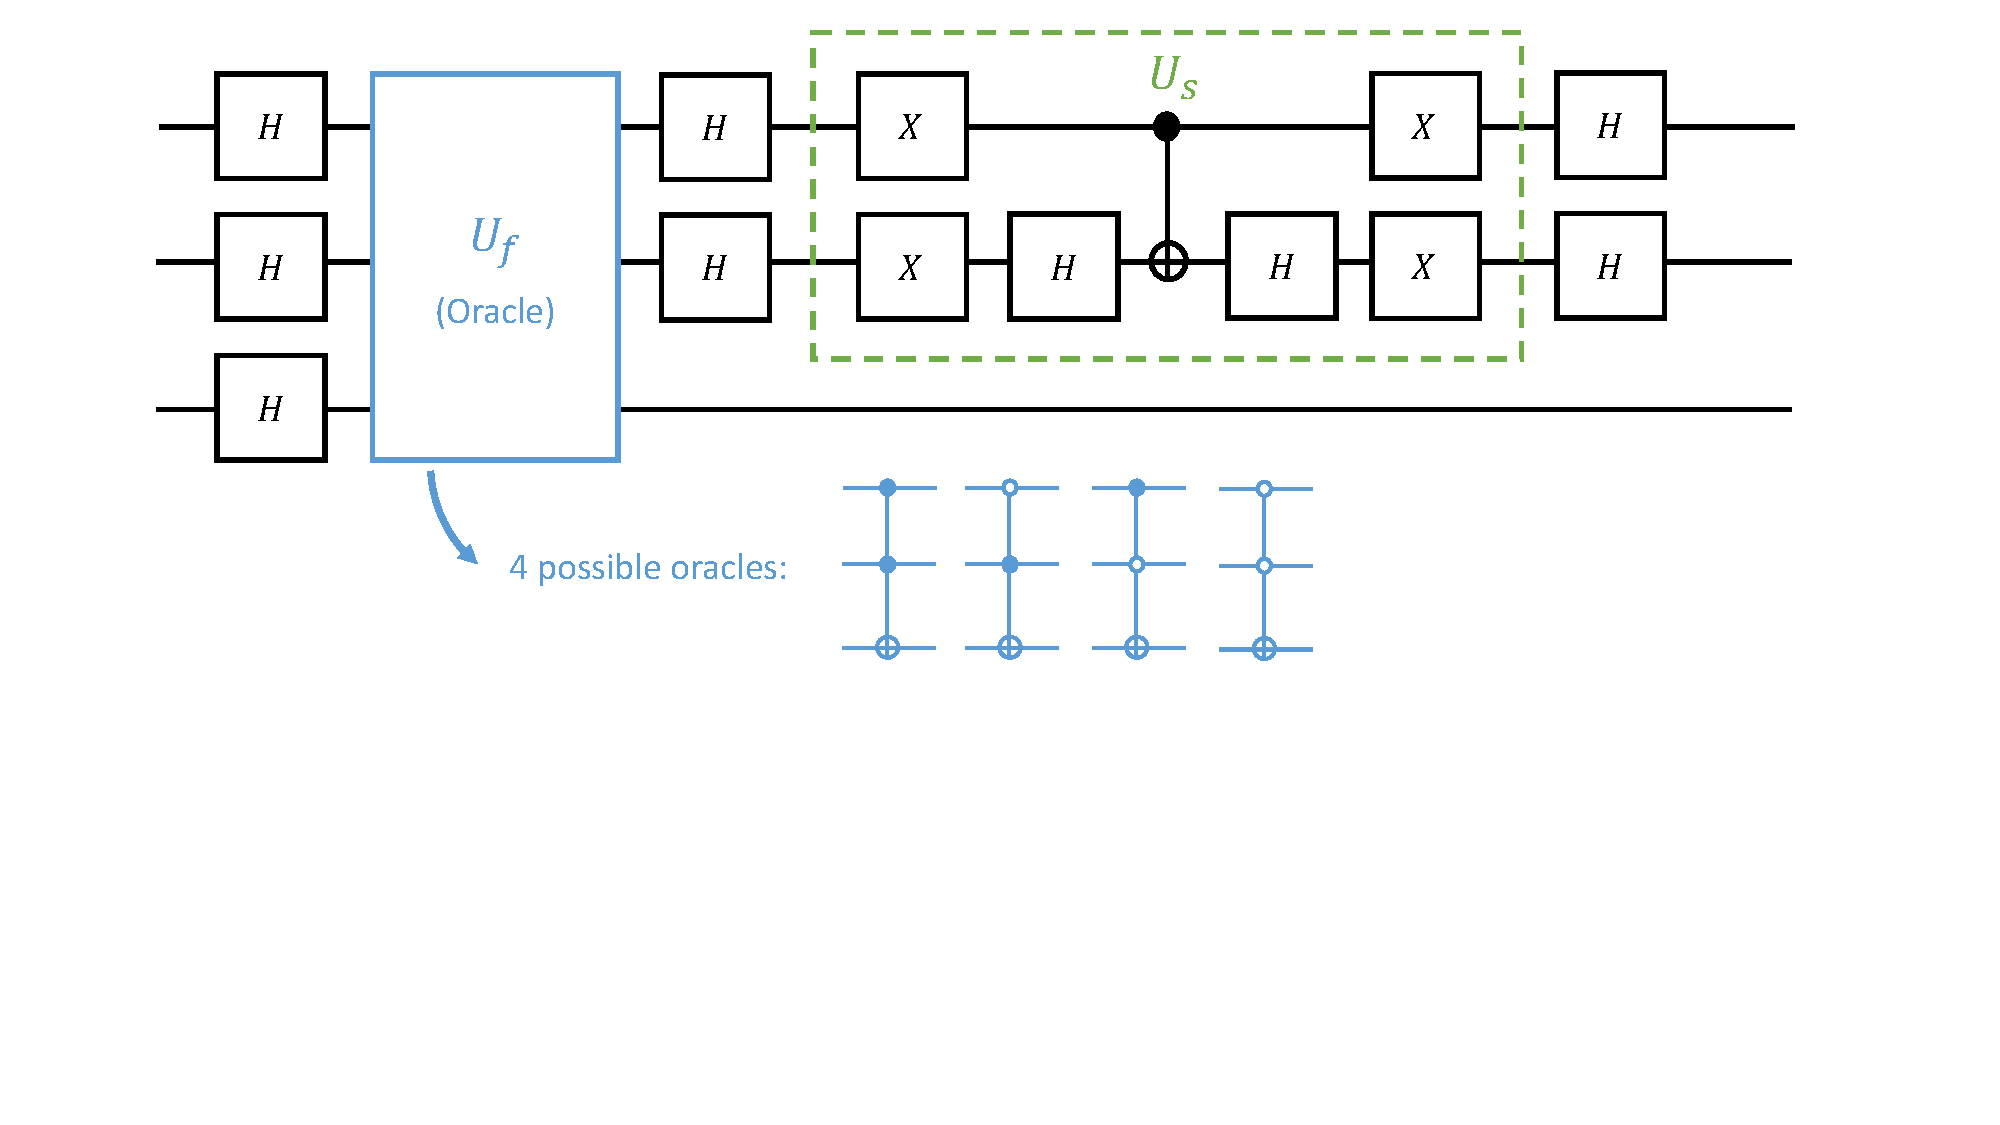
\includegraphics[width=.97\textwidth]{Lecture7Figs/gcircex.pdf}
    \label{fig:search_item}
\end{figure}
\newline
As you can see, there are four different possible oracles, corresponding to the state we are searching for. On your pset you will be tasked with verifying that each of these oracles result in a different output states.

\subsection{Further Reading}
To see how the algorithm can be implemeted in a hybrid system (i.e. one with classical memory) and how the algorithm acts when there are multiple winner states in the list of items, read chapter 6 of \textit{Quantum Computation and Quantum Information}, by Nielsen and Chuang.
\end{document}